\documentclass[fleqn, a4paper, 12pt, twoside]{article}

\newcounter{recitationcount} %creates a new counter for recitation numbers (must be executed before exsheets is loaded)
\newcommand\recitation{\refstepcounter{recitationcount}}

\usepackage[counter-within = recitationcount]{exsheets} %question and solution environments
\usepackage{amsmath, amssymb, amsthm} %standard AMS packages
\usepackage{esint} %integral signs
\usepackage{marginnote} %marginnotes
\usepackage{gensymb} %miscellaneous symbols
\usepackage{commath} %differential symbols
\usepackage{xcolor} %colours
\usepackage{cancel} %cancelling terms
\usepackage[free-standing-units]{siunitx} %formatting units
\usepackage{tikz, pgfplots} %diagrams
	\usetikzlibrary{calc, hobby, patterns, intersections, angles, quotes, spy}
\usepackage{graphicx} %inserting graphics
\usepackage{epstopdf} %converting and inserting eps graphics
\usepackage{hyperref} %hyperlinks
\usepackage{datetime} %date and time
\usepackage{ulem} %underline for \emph{}
\usepackage{xfrac, lmodern} %inline fractions
\usepackage{enumerate, enumitem} %numbered lists
\usepackage{float} %inserting floats
\usepackage[american voltages]{circuitikz} %circuit diagrams
\usepackage{pdflscape} %pages in landscape orientation
\usepackage{setspace} %double spacing
\usepackage{microtype} %micro-typography
\usepackage{listings} %formatting code
	\lstset{language=Matlab}
	\lstdefinestyle{standardMatlab}
	{
		belowcaptionskip=1\baselineskip,
		breaklines=true,
		frame=L,
		xleftmargin=\parindent,
		language=C,
		showstringspaces=false,
		basicstyle=\footnotesize\ttfamily,
		keywordstyle=\bfseries\color{green!40!black},
		commentstyle=\itshape\color{purple!40!black},
		identifierstyle=\color{blue},
		stringstyle=\color{orange},
	}
\usepackage{algpseudocode} %algorithms
\usepackage{algorithm} %algorithms

\renewcommand{\marginfont}{\scriptsize \color{blue}}

\newcommand\numberthis{\addtocounter{equation}{1}\tag{\theequation}} %adds numbers to specific equations in non-numbered list of equations

\theoremstyle{definition}
\newtheorem{example}{Example}
\newtheorem{definition}{Definition}

\theoremstyle{theorem}
\newtheorem{theorem}{Theorem}
\newtheorem{law}{Law}

\newcommand{\curl}{\mathrm{curl\,}}

\newcommand{\divergence}{\mathrm{div\,}}

\makeatletter
\@addtoreset{section}{part} %resets section numbers in new part
\makeatother

\newcommand\blfootnote[1]{%
	\begingroup
	\renewcommand\thefootnote{}\footnote{#1}%
	\addtocounter{footnote}{-1}%
	\endgroup
}

\renewcommand{\tilde}{\widetilde}

\RenewQuSolPair{question}[name=Recitation \therecitationcount\ -- Exercise]{solution}[name=Recitation \therecitationcount\ -- Solution]

\SetupExSheets{solution/print = true} %prints all solutions by default

%opening
\title{Harmonic Analysis : Recitations}
\author{Aakash Jog}
\date{2015-16}

\begin{document}

\maketitle
%\setlength{\mathindent}{0pt}

\blfootnote
{	
	\begin{figure}[H]
		
\includegraphics[height = 12pt]{cc.eps}
		\includegraphics[height = 12pt]{by.eps}
		\includegraphics[height = 12pt]{nc.eps}
		
\includegraphics[height = 12pt]{sa.eps}
	\end{figure}
	This work is licensed under the Creative Commons Attribution-NonCommercial-ShareAlike 4.0 International License. To view a copy of this license, visit \url{http://creativecommons.org/licenses/by-nc-sa/4.0/}.
} %CC-BY-NC-SA license

\tableofcontents

\newpage
\section{Instructor Information}

\textbf{Yaron Yeger}\\
~\\
Office: Shenkar Physics 201\\
E-mail: \href{mailto:yaronyeg@mail.tau.ac.il}{yaronyeg@mail.tau.ac.il}\\

\newpage
\part{Fourier Series}

\recitation
\section{Fourier Series}

\begin{definition}[Real Fourier series]
	Let $f : [-L,L] \in \mathbb{C}$ be a piecewise continuous function.\\
	The series
	\begin{align*}
		f(x) & \approx \frac{a_0}{2} + \sum\limits_{n = 1}^{\infty} \left( a_n \cos(n x) + b_n \sin(n x) \right)
	\end{align*}
	is called the Fourier series of $f(x)$, where
	\begin{align*}
		a_0 & = \frac{1}{L} \int\limits_{-L}^{L} f(x) \dif x           \\
		a_n & = \frac{1}{L} \int\limits_{-L}^{L} f(x) \cos(n x) \dif x \\
		b_n & = \frac{1}{L} \int\limits_{-L}^{L} f(x) \sin(n x) \dif x
	\end{align*}
\end{definition}

\begin{theorem}
	If $f(x)$ is an even function, then the appropriate Fourier series is
	\begin{align*}
		f(x) & \approx \frac{a_0}{2} + \sum\limits_{n = 1}^{\infty} a_n \cos(n x)
	\end{align*}
	If $f(x)$ is an odd function, then the appropriate Fourier series is
	\marginnote
	{
		If $f(x)$ is odd, its graph always passes through the origin.
		Therefore, it can be represented by a summation of sine functions, which also pass through the origin, and there is no need for a term, i.e. $\frac{a_0}{2}$, to change its position at the origin.
	}
	\begin{align*}
		f(x) & \approx \sum\limits_{n = 1}^{\infty} a_n \sin(n x)
	\end{align*}
\end{theorem}

\begin{definition}[Complex Fourier series]
	Let $f : [-L,L] \in \mathbb{C}$ be a piecewise continuous function.\\
	The series
	\begin{align*}
		f(x) & \approx \sum\limits_{n = -\infty}^{\infty} c_n e^{i n x}
	\end{align*}
	is called the complex Fourier series of $f(x)$, where
	\begin{align*}
		c_n & = \frac{1}{2 L} \int\limits_{-L}^{L} f(x) e^{-i n x} \dif x
	\end{align*}
\end{definition}

\begin{question}
	Calculate the real Fourier series of
	\begin{align*}
		f(x) & = 2 x - 2 \pi
	\end{align*}
\end{question}

\begin{solution}
	As $x$ is an odd function, the real Fourier series of $x$, in the interval $[-\pi,\pi]$ is
	\begin{align*}
		x & \approx \sum\limits_{n = 1}^{\infty} b_n \sin(n x)
	\end{align*}
	where
	\begin{align*}
		b_n & = \frac{1}{\pi} \int\limits_{-\pi}^{\pi} x \sin(n x) \dif x                                                                                                   \\
                    & = \frac{1}{\pi} \left. \left( x \int \sin(n x) \dif x - \int 1 \left( \int \sin(n x) \dif x \right) \dif x \right) \right|_{-\pi}^{\pi}                      \\
                    & = \frac{1}{\pi} \left. \left( -\frac{x \cos(n x)}{n} \right) \right|_{-\pi}^{\pi} + \frac{1}{\pi} \int\limits_{-\pi}^{\pi} \frac{\cos(n x)}{n} \dif x        \\
                    & = \frac{1}{\pi} \left( -\frac{\pi \cos(n \pi) + \pi \cos(-n \pi)}{n} \right) + \frac{1}{\pi} \cancelto{0}{\left. \frac{\sin(n x)}{n^2} \right|_{-\pi}^{\pi}} \\
                    & = -\frac{\cos(n \pi) + \cos(n \pi)}{n}                                                                                                                       \\
                    & = -2 \frac{\cos(n \pi)}{n}                                                                                                                                   \\
                    & = -2 \frac{(-1)^{n}}{n}
	\end{align*}
	Therefore,
	\begin{align*}
		x & \approx 2 \sum\limits_{n = 1}^{\infty} \frac{(-1)^{n + 1}}{n} \sin(n x)
	\end{align*}
	Therefore,
	\begin{align*}
		2 x - 2 \pi & \approx \left( 4 \sum\limits_{n = 1}^{\infty} \frac{(-1)^{n + 1}}{n} \sin(n x) \right) - 2 \pi \\
	\end{align*}
\end{solution}

\end{document}
